% 05-results.tex -- draft from the battery of 17/11 (540 runs).
% Numbers: medians of 10 repetitions (k6 summaries, confirmed by per-request
% percentiles). Re-check every number against paper/tables before submission.
% Energy paragraphs wait for the halt-polling decision.

\section{RQ1: What Does Each Mesh Cost?}
\label{sec:rq1}

\paragraph{Throughput}
\Cref{tab:sat} reports the maximum throughput each configuration sustains
within the SLO. Every mesh reduces it, but by very different amounts. Ambient
L4 keeps 78--85\% of the no-mesh throughput on all three applications. At the
other end, Cilium sustains only 21\% on the echo benchmark, and the Istio
sidecar 30\%. On Hotel Reservation, the three configurations that route
traffic through a shared L7 proxy (the Ambient waypoint, Cilium's per-node
Envoy) and Linkerd all fall to 47\%, below the Istio sidecar (54\%).

\begin{table}[t]
  \centering
  \caption{Maximum SLO-compliant throughput (req/s) and fraction of the
           no-mesh baseline.}
  \label{tab:sat}
  \small
  \begin{tabular}{@{}lrrr@{}}
    \toprule
         & Echo & OB & HR \\
    \midrule
    B    & 14012        & 1274       & 2287 \\
    IA4  & 11688 (83\%) & 990 (78\%) & 1953 (85\%) \\
    IA7  & 8208 (59\%)  & 953 (75\%) & 1067 (47\%) \\
    LK   & 5253 (37\%)  & 793 (62\%) & 1068 (47\%) \\
    IS   & 4202 (30\%)  & 793 (62\%) & 1233 (54\%) \\
    CI   & 2939 (21\%)  & 915 (72\%) & 1067 (47\%) \\
    \bottomrule
  \end{tabular}
\end{table}

\paragraph{Tail latency}
\Cref{fig:p99load} shows p99 latency against load, and \cref{tab:p99} the
medians with significance against the baseline. At 90\% load, Ambient L4 adds
the least: +60\% on echo, +62\% on OB, and +54\% on HR. The Istio sidecar is
the worst on OB, the application with the deepest call graph (11 internal calls
per request, 10.4 of them across nodes; \cref{sec:rq3}), where its p99 grows by
+1025\% (11.9 to 133.7\,ms). Cilium is the worst on echo (+799\%), even though
the echo chain has a single internal hop. Linkerd is consistently better than
the Istio sidecar (+463\% vs.\ +1025\% on OB) although both place a proxy in
every pod. The ranking is the same at 60\% load. The p99.9 follows it: at 90\% load the
Istio sidecar multiplies the baseline p99.9 by 8.4 on OB and Linkerd by 5.4,
while Ambient L4 stays within 1.2--1.6$\times$ on all three applications;
Cilium reaches 6.8$\times$ on echo. The differences are not marginal.
Kruskal--Wallis rejects equal p99 across configurations for every application
and load ($p<10^{-9}$), all 45 mesh-versus-baseline comparisons remain
significant after Holm correction (largest adjusted $p = 0.0009$), and Cliff's
$\delta = 1$ in every case: every repetition of every mesh is slower than every
repetition of the baseline.

\begin{figure}[t]
  \centering
  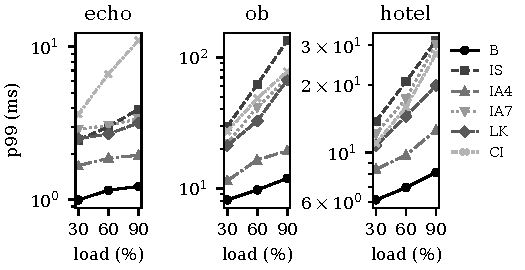
\includegraphics[width=\columnwidth]{figs/p99_carga.pdf}
  \caption{p99 latency vs.\ load level (median of 10 runs).}
  \label{fig:p99load}
\end{figure}

\begin{table*}[t]
  \centering
  \caption{p99 latency (ms), median of 10 runs. $^{*}$: different from B
           (Mann--Whitney, Holm-corrected, $p<0.05$).}
  \label{tab:p99}
  \small
  % gerado por analysis/20_estatistica.py; não editar à mão
\begin{tabular}{lrrrrrrrrr}
\toprule
Config. & echo 30\% & echo 60\% & echo 90\% & hotel 30\% & hotel 60\% & hotel 90\% & ob 30\% & ob 60\% & ob 90\% \\
\midrule
No mesh & 1.00 & 1.15 & 1.22 & 6.14 & 6.97 & 8.14 & 8.14 & 9.70 & 11.88 \\
Istio sidecar & 2.46$^{*}$ & 3.00$^{*}$ & 3.91$^{*}$ & 13.76$^{*}$ & 20.67$^{*}$ & 31.46$^{*}$ & 29.58$^{*}$ & 61.73$^{*}$ & 133.70$^{*}$ \\
Istio ambient (L4) & 1.67$^{*}$ & 1.87$^{*}$ & 1.95$^{*}$ & 8.39$^{*}$ & 9.74$^{*}$ & 12.54$^{*}$ & 11.40$^{*}$ & 16.44$^{*}$ & 19.30$^{*}$ \\
Istio ambient + waypoint & 2.88$^{*}$ & 3.07$^{*}$ & 3.38$^{*}$ & 12.11$^{*}$ & 17.35$^{*}$ & 30.35$^{*}$ & 21.95$^{*}$ & 41.51$^{*}$ & 69.31$^{*}$ \\
Linkerd & 2.51$^{*}$ & 2.69$^{*}$ & 3.17$^{*}$ & 10.73$^{*}$ & 14.49$^{*}$ & 19.88$^{*}$ & 21.10$^{*}$ & 32.56$^{*}$ & 66.88$^{*}$ \\
Cilium (WG + L7) & 3.63$^{*}$ & 6.64$^{*}$ & 10.97$^{*}$ & 10.96$^{*}$ & 15.91$^{*}$ & 27.40$^{*}$ & 27.16$^{*}$ & 48.39$^{*}$ & 77.48$^{*}$ \\
\bottomrule
\end{tabular}
% p99_ms: mediana de 10 repetições; * = diferente da B (Mann-Whitney, Holm, p<0,05)

\end{table*}

\paragraph{CPU and memory}
\Cref{fig:resources} breaks CPU down by component, normalized per
1{,}000\,req/s. At 90\% load, Ambient L4 adds the least CPU (+33\% to +61\%
depending on the application), while Cilium adds the most (+93\% on OB and
+306\% on echo). The Istio sidecar adds +215\% on echo and +116\% on HR.
The dominant component differs by design: the per-pod proxies for the Istio
sidecar and Linkerd (on OB, 4.8 and 3.6 cores per 1{,}000\,req/s), ztunnel
for Ambient L4 (2.1), ztunnel and the waypoint in similar shares for IA7 (1.3
and 1.9), and, for Cilium, the agent and the per-node Envoy in equal parts (2.6
and 3.1). Memory is mostly a fixed cost: the Istio sidecars hold 1.8\,GiB
across the 32 application pods (about 57\,MiB each), against 0.22\,GiB for
Linkerd's proxies (about 7\,MiB each); ztunnel uses about 100\,MiB in total and
the three waypoints 375\,MiB. The Istio and Linkerd control planes add about
165 and 145\,MiB on the control-plane node.

\begin{figure}[t]
  \centering
  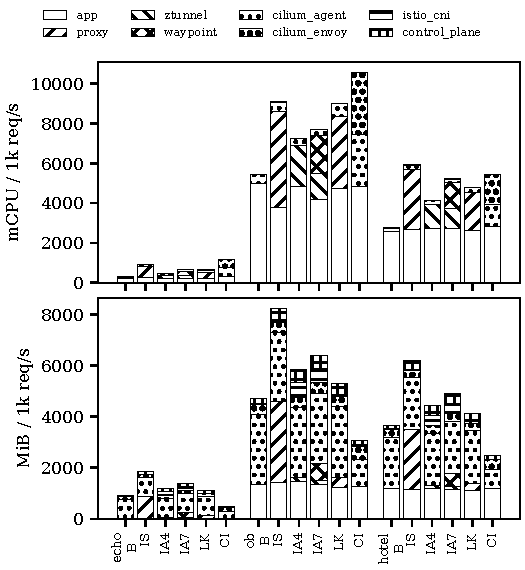
\includegraphics[width=\columnwidth]{figs/recursos.pdf}
  \caption{CPU and memory per 1{,}000\,req/s by component, at 90\% load.}
  \label{fig:resources}
\end{figure}

\paragraph{Energy}
\todo{Pending the halt-polling check. State the common idle baseline (idle
power of B), J/req per mesh, and the virtualization caveat.}

\paragraph{Variability}
Results are stable across repetitions: the coefficient of variation of p99
never exceeds 0.22 (Linkerd on OB at 90\% load). Five of the 540 runs, all on
HR, had error rates between 0.13\% and 0.38\%, and one dropped 37 requests;
all are below the 1\% threshold and are kept.

\section{RQ2: Where Does the Cost Come From?}
\label{sec:rq2}

We profiled every configuration at 60\% load on echo and OB
(\cref{sec:design}) and attribute to the data plane all samples of the proxy
processes (Envoy, \texttt{linkerd2-proxy}, ztunnel, the Cilium agent) plus any
kernel stack that runs WireGuard or an eBPF program. \Cref{fig:perfil}
breaks this CPU down per request and \cref{tab:perfil} summarizes it.

\paragraph{What each data plane spends}
On OB, the baseline spends 0.64\,ms of CPU per request in its data plane (the
Cilium CNI's eBPF programs). The Istio sidecar spends 5.5\,ms, of which 61\% is
HTTP/2 framing and header compression (\texttt{nghttp2}): with 11 internal
calls per request, each crossing two sidecars, protocol processing dominates,
as MeshInsight found for an older Envoy~\cite{zhu2023meshinsight}. Ambient L4
spends 2.6\,ms, almost half of it (47\%) in TLS inside ztunnel and no L7
parsing; adding the waypoint (IA7) raises it to 4.2\,ms, split between the
waypoint's HTTP processing (39\%) and ztunnel's TLS (31\%). Linkerd spends
4.6\,ms; because its proxy is distributed without symbols, 46\% of it can only
be attributed to the proxy as a whole, and 13\% is kernel networking. Every
mesh also multiplies kernel crossings: on OB, the proxy processes make 191
(IS) to 329 (CI) system calls and 58 to 152 context switches per request,
against 48 and 31 in the baseline.

\paragraph{Why Cilium is the slowest on echo}
On echo, Cilium spends 0.92\,ms of data-plane CPU per request, 9.6$\times$ the
baseline and 1.6$\times$ the Istio sidecar, although the request crosses a
single internal hop. Every request is redirected to the per-node Envoy by the
L7 rule on both nodes, is encrypted by WireGuard (14\% of the total), and makes
the Cilium agent spend almost as much CPU as Envoy itself (36\,s against 39\,s
over the profiling window). It also has the most context switches per request
(27, against 12 for the sidecar). We could not resolve the agent's symbols, so
we cannot say which agent function consumes this time.

\paragraph{Why the Istio sidecar is the slowest on OB}
On OB, Cilium spends even more CPU per request than the sidecar (7.2 against
5.5\,ms), yet its p99 is lower (77 against 134\,ms at 90\% load). The
difference is where the work runs. The sidecar's cost follows the frontend,
which issues all 11 internal calls through its own proxy, so it accumulates on
the frontend's node: at 90\% load that worker is 76\% utilized with the
sidecar and 68\% with Cilium, whose per-node Envoys spread L7 work over the
nodes that receive the calls. Tail latency is set by queueing on that node,
which is the mechanism behind the queueing term of our model (\cref{sec:rq3}).

\begin{figure}[t]
  \centering
  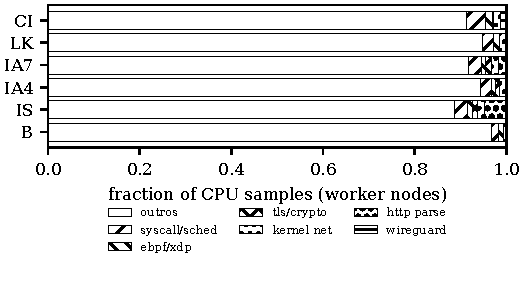
\includegraphics[width=\columnwidth]{figs/perfil.pdf}
  \caption{Data-plane CPU per request by category, at 60\% load (sum of the
           three workers).}
  \label{fig:perfil}
\end{figure}

\begin{table}[t]
  \centering
  \caption{Data-plane CPU per request at 60\% load, share spent in
           cryptography (TLS and WireGuard) and HTTP/gRPC processing, and
           context switches (cs) and system calls (sys) of the proxy
           processes per request.}
  \label{tab:perfil}
  \small
  \setlength{\tabcolsep}{3pt}
  % gerado por analysis/50_perfil.py
\begin{tabular}{llrrrrr}
\toprule
App & Config. & CPU ($\mu$s/req) & TLS+WG & HTTP & cs/req & sys/req \\
\midrule
echo & B & 95 & 0\% & 0\% & 7.6 & 12.5 \\
echo & IS & 584 & 10\% & 52\% & 12.4 & 36.8 \\
echo & IA4 & 240 & 24\% & 6\% & 12.7 & 29.9 \\
echo & IA7 & 418 & 22\% & 30\% & 15.7 & 46.9 \\
echo & LK & 389 & 0\% & 0\% & 14.0 & 30.8 \\
echo & CI & 916 & 14\% & 0\% & 26.7 & 61.7 \\
ob & B & 641 & 0\% & 0\% & 31.0 & 47.7 \\
ob & IS & 5485 & 11\% & 61\% & 58.1 & 190.6 \\
ob & IA4 & 2591 & 47\% & 10\% & 82.1 & 264.2 \\
ob & IA7 & 4206 & 31\% & 39\% & 68.9 & 302.9 \\
ob & LK & 4624 & 0\% & 0\% & 71.4 & 219.5 \\
ob & CI & 7213 & 16\% & 0\% & 151.8 & 329.2 \\
\bottomrule
\end{tabular}

\end{table}

\section{RQ3: Can the Overhead Be Predicted?}
\label{sec:rq3}

\paragraph{Model}
We model the latency added by a mesh as
\begin{equation}
  \Delta L = P_{m}(a)\, c_{m} + q_{m}\, \frac{\rho_{\text{hot}}}{1-\rho_{\text{hot}}},
  \label{eq:model}
\end{equation}
where $P_m(a)$ is the number of proxy traversals that mesh $m$ adds to a
request of application $a$, $c_m$ is the cost of one traversal,
$\rho_{\text{hot}}$ is the measured CPU utilization of the busiest worker, and
$q_m$ scales the queueing term. $P_m(a)$ comes from the call graph measured
with Istio telemetry: echo makes 1 internal call per request (across nodes),
OB 11 (10.4 across nodes), and HR 3.8 (1.0 across nodes, 2.8 on the same
node). A sidecar mesh adds two traversals per call, ztunnel one per node
crossed, and the waypoint one more per L7 call. We fit $c_m$ and $q_m$ by
non-negative least squares on echo and OB and predict HR, which is held out.

\paragraph{Results}
\Cref{tab:model} shows the prediction error. For Ambient L4 the model predicts
the p99 of HR with 11\% error (22\% for the mean), and yields a cost of
72--120\,\textmu s per ztunnel traversal. For the other meshes it does not
generalize: errors range from 82\% (Linkerd) to 140\% (Ambient with waypoint)
on p99. For the Istio sidecar and the waypoint, the fit assigns the whole
overhead to the queueing term ($c_m = 0$): on OB, the frontend and its proxy
saturate the node that hosts them, and the per-hop cost cannot be separated
from queueing on that node. We therefore read RQ3 as a partial answer. A
per-traversal model suffices when the data plane is light (L4), but for L7
data planes tail latency is governed by the utilization of the busiest node,
which depends on placement as much as on the mesh. Leaving one load level out
instead of one application gives p99 errors from 27\% (Ambient L4) to 111\%
(Istio sidecar), which confirms this reading.

\begin{table}[t]
  \centering
  \caption{Model parameters and prediction error on HR (held out). $P$:
           proxy traversals per request; $c$: fitted cost per traversal;
           LOLO: error when leaving one load level out.}
  \label{tab:model}
  \small
  \setlength{\tabcolsep}{3pt}
  % generated by analysis/41_modelo_x.py
\begin{tabular}{lrrrrrr}
\toprule
Config. & $c_p$ ($\mu$s) & $c_x$ ($\mu$s) & $q$ (ms) & err.\ HR & err.\ place. & err.\ $X_{\max}$ \\
\midrule
IS & 0 & 0 & 35.0 & 135\% & 40\% & 4\% \\
IA4 & 120 & 0 & 3.8 & 11\% & -- & 8\% \\
IA7 & 0 & 0 & 42.6 & 138\% & 27\% & 17\% \\
LK & 56 & 0 & 21.4 & 82\% & -- & 9\% \\
CI & 798 & 0 & 23.8 & 140\% & -- & 7\% \\
CI4 & 0 & 277 & 2.8 & 13\% & -- & -- \\
\bottomrule
\end{tabular}

\end{table}

\section{RQ4: Which Mesh Should I Use?}
\label{sec:rq4}

\Cref{tab:guide} condenses our results into a decision guide. Two observations
cut across it. First, the cheapest mesh is the one that does the least per
request: Ambient L4 avoids L7 parsing entirely and is the best option on every
metric we measured. Second, for L7 data planes, where the work runs matters as
much as how much work there is: shared proxies and services with a high
fan-out concentrate CPU on a few nodes, and the busiest node sets the tail, so
their placement should be part of capacity planning.

\begin{table}[t]
  \centering
  \caption{Decision guide. Evidence at 90\% load unless stated otherwise.}
  \label{tab:guide}
  \footnotesize
  \setlength{\tabcolsep}{3pt}
  \begin{tabular}{@{}p{0.27\columnwidth}p{0.17\columnwidth}p{0.5\columnwidth}@{}}
    \toprule
    Need & Choose & Evidence \\
    \midrule
    mTLS and L4 policy only & IA4 & lowest p99 increase (+54 to +62\%), 78--85\% of
      no-mesh throughput, least CPU; no L7 parsing (\cref{sec:rq2}) \\
    L7 policy, deep call graphs & LK or IA7 & p99 on OB: +463\% (LK) and +483\% (IA7)
      vs.\ +1025\% (IS) \\
    L7 on a high fan-out service & IA7, waypoint off the hot node & the sidecar
      concentrates the fan-out on one node (76\% utilized) \\
    Smallest memory footprint & IA4 or LK & ztunnel 100\,MiB in total; Linkerd
      7\,MiB per pod vs.\ 57\,MiB for Istio sidecars \\
    Already on Cilium, few L7 rules & CI, scoped L7 rules & highest data-plane CPU per
      request (0.92\,ms on echo); node Envoy, agent and WireGuard on every request \\
    \bottomrule
  \end{tabular}
\end{table}

\section{Threats to Validity}
\label{sec:threats}

\paragraph{Single host}
All VMs share one host, memory bus, and last-level cache. We mitigate this by
pinning every vCPU to a dedicated physical thread and by validating against
MeshInsight (\cref{sec:validation}), but absolute numbers will differ on
physical clusters.

\paragraph{Energy under virtualization}
RAPL measures the whole package, including the hypervisor. We found that KVM
halt-polling makes idle-heavy configurations draw more power than their
in-guest CPU use predicts.\todo{finalize after the halt-polling check}

\paragraph{Ordering}
Runs are randomized within each configuration, but configurations ran in
blocks. An interleaved control experiment (B and IS alternated in blocks)
reproduced the same power difference at the same temperatures, which rules out
time of day and temperature as its cause.

\paragraph{Versions and defaults}
Meshes evolve quickly; we pin versions and use default proxy settings, which
may not match tuned production deployments.

\paragraph{Applications}
Two benchmark applications and a microbenchmark cannot represent every call
graph; Hotel Reservation keeps most of its calls on the same node under our
placement, which favors node-level proxies.

\section{Conclusion}
\label{sec:conclusion}

We compared six service-mesh configurations on the same testbed, with open-loop
load and the same absolute request rates for all of them. Istio Ambient in L4
mode is the cheapest mesh on every metric: it keeps 78--85\% of the no-mesh
throughput and adds 54--62\% to p99 at 90\% load, while the L7 data planes add
144--1025\%. Profiling shows where the difference comes from: HTTP/2 processing for
the Istio sidecar, TLS for ztunnel, and the per-node Envoy, the agent, and
WireGuard for Cilium. Beyond per-request cost, the tail of L7 meshes is set by
the busiest node, which a per-hop model cannot capture and placement can
change. We release the testbed and data so that these results can be
reproduced and extended.
